\section{FrontPageの設計}
my\_helpをよりよくするための設計を示す.
各学生のFrontPage,各helpのページに分けて,実装すると便利になる理由と共に記述している.

\begin{figure}[htbp]
\begin{center}
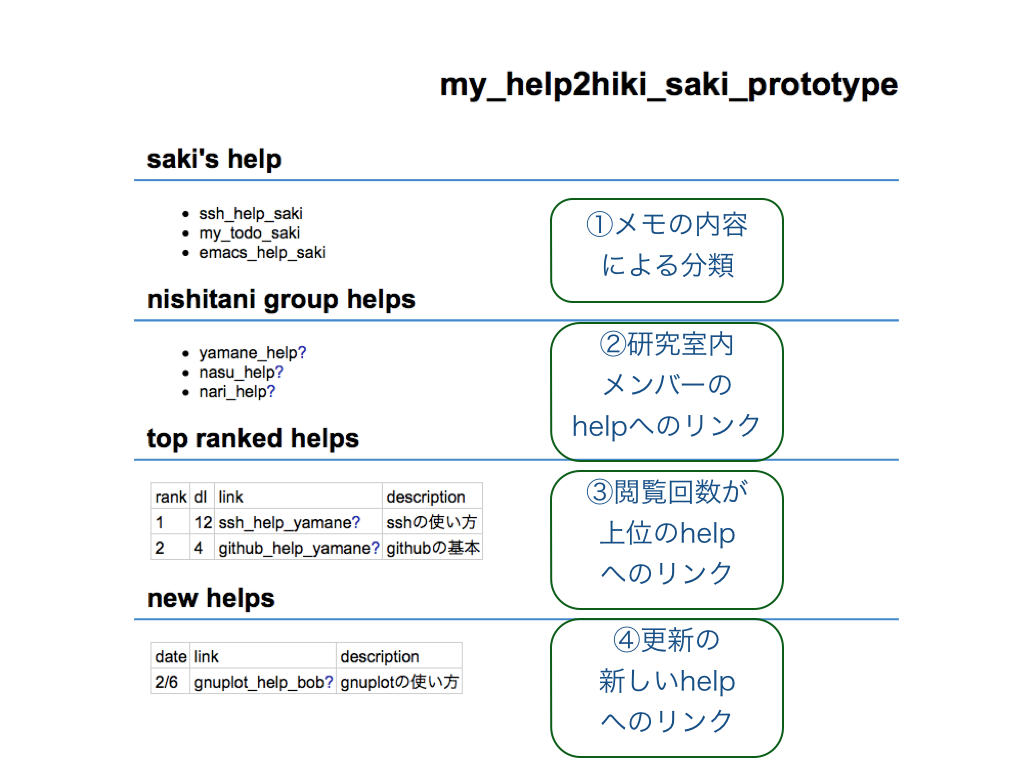
\includegraphics[width=6.0cm,bb=0 0 600 800]{my_help2hiki_saki.014.png}
\caption{FrontPage}
\label{default}\end{center}\end{figure}

\begin{itemize}
\item 1.メモの内容による分類
\end{itemize}
\begin{description}
\item 研究室内の所属学生の利用するハードウェア,ソフトウェアは同じものが多い.
例えば,西谷研究室ではハードウェアは全員がmacを使い,プログラム作成はターミナル,
hiki文書の作成にはmiというソフトを使用している.
それぞれのハードウェア,ソフトウェアに関するhelpを分類分けしておくことで,
調べたいことに関してのhelpを探しやすくすることができる.\\
\end{description}
\newpage
\begin{itemize}
\item 2.研究室内のメンバーのhelpへのリンク
\end{itemize}
\begin{description}
\item 同研究室の他学生のFrontPageへのリンクを作る.
同回のメンバーが書いたメモを見たい,先輩のメモを見たい,他メンバーの研究を知りたい.
そのときの目的に応じて閲覧するhelpを選ぶことができる.\\
\end{description}

\begin{itemize}
\item 3.閲覧回数が上位のhelpへのリンク
\end{itemize}
\begin{description}
\item 閲覧回数の多い,研究室内の学生が見た回数の多いものへのリンクを作る.
研究室に入ってばかりで分からないことが多いときにこのhelpを見れば,研究室のことが理解できる.
知らなくても支障はないが,知っておくと便利な豆知識を得ることが期待される.\\
\end{description}

\begin{itemize}
\item 4.更新の新しいhelpへのリンク
\end{itemize}
\begin{description}
\item 更新が新しいものを表示しておくことで,メンバーが得た最新の知識を得やすくなる.
また,他メンバーがどのような研究を進めているか,どのようなことを調べてたのかを知ることができ,自分の研究の進め方の参考にすることができる.
\end{description}

\newpage
\begin{figure}[htbp]\begin{center}
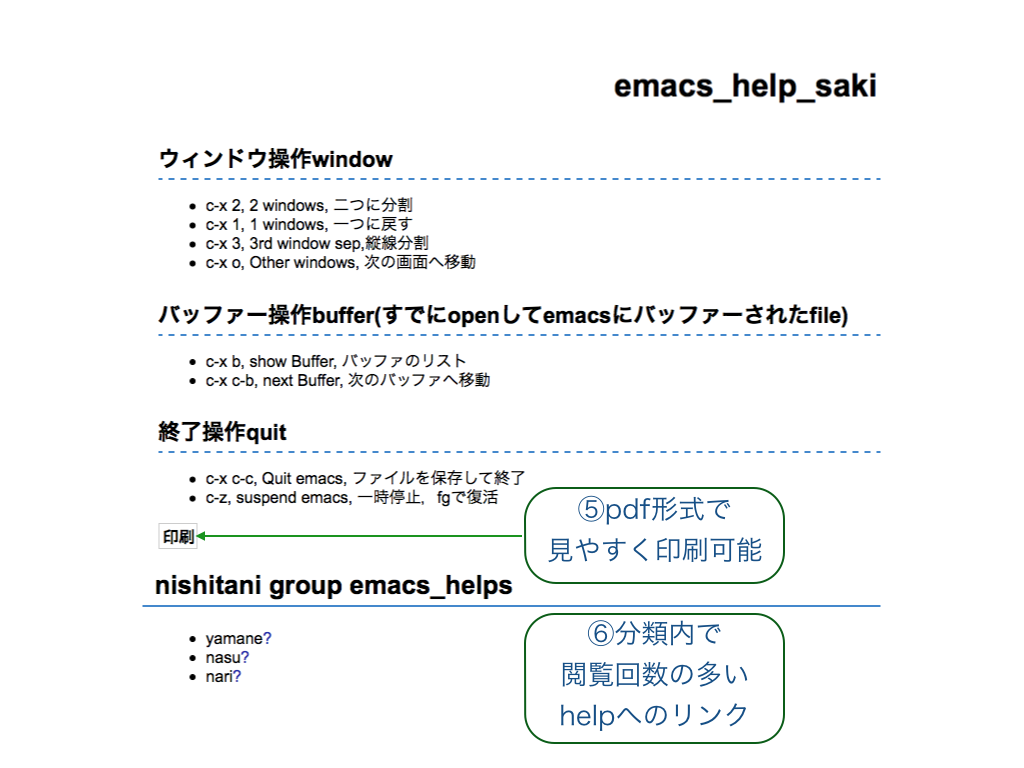
\includegraphics[width=6cm,bb=0 0 600 800]{my_help2hiki_saki.015.png}
\caption{例 emacs\_helpから一部抜粋}
\label{default}\end{center}\end{figure}

\begin{itemize}
\item 5. pdf形式で見やすく印刷可能
\end{itemize}
\begin{description}
\item 紙媒体で持ち歩くことを可能にするために,pdf形式に変換することで見やすくしたhelpを印刷することができる.
emacs\_helpを例にして考える.このhelpはターミナルでemacsを使うときのキーバインドを表している.
ターミナルを利用していると,このhelpを開きながら操作することは手間がかかる.
そこで見やすくしたhelpを紙に印刷することでこの手間を省くことができる.
西谷研究室ではhikiからlatex(pdf形式への変換を可能にするソフト)への変換システム,hiki2latexがあるので,作成可能だと考えられる.\\
\end{description}

\begin{itemize}
\item 6.分類内で閲覧回数の多いhelpへのリンク
\end{itemize}
\begin{description}
\item 分類内で閲覧回数の多いhelpは他メンバーの多くが得た知識なので,
知っておくべき知識であるといえる.
自分がその分類内で分からないことを解決する手がかりになることが期待される
\end{description}
